%\section{Aprendizaje automático} 

%\begin{frame}
%\frametitle{Aprendizaje Automático}
%\graphictocap
%\end{frame}



%\subsection{Introducción}

%\begin{myframe}
%\frametitle{Reconocimiento de gestos = Clasificación}
%\centering
%\esquemaclasificacion{0.8}
%\end{myframe}

%\begin{frame}
%\frametitle{Clasificación: Perspectiva Geométrica}
%\centering
%\begin{columns}
%\begin{column}{0.7\textwidth}
%\includegraphics<1>[width=\textwidth]{aprendizaje/clases3}
%\includegraphics<2>[width=\textwidth]{aprendizaje/voronoi3}
%\end{column}
%\begin{column}{0.3\textwidth}
%
%\begin{block}{Ejemplares}
%  Puntos en $ \mathbb{R}^d$
%\end{block}
%
%\begin{block}{Clases}
%  Superficies de separación en $ \mathbb{R}^d$
%\end{block}
%
%\begin{block}{Hipótesis}
%  La asignación de clases es una función suave
%\end{block}
%
%\end{column}
%
%\end{columns}
%\end{frame}



%\begin{frame}
%\frametitle{Modelo: El Perceptrón}
%\centering
%
%\begin{columns}
%
%\begin{column}{0.31\textwidth}
%
%\begin{block}{Hiperplano}
%$  h(\ve{x}) = \ve{w} \cdot \ve{x} =0$
%\end{block}
%
%\begin{block}{Separación}
%    $\ve{w} \cdot \ve{x} > 0 \rightarrow $ Clase + \\
%    $ \ve{w} \cdot \ve{x} < 0 \rightarrow $ Clase - \\
%\end{block}
%
%\begin{block}{Modelo}
%  Parámetro: $\ve{w}$.
%\end{block}
%
%\end{column}
%
%\begin{column}{0.7\textwidth}
%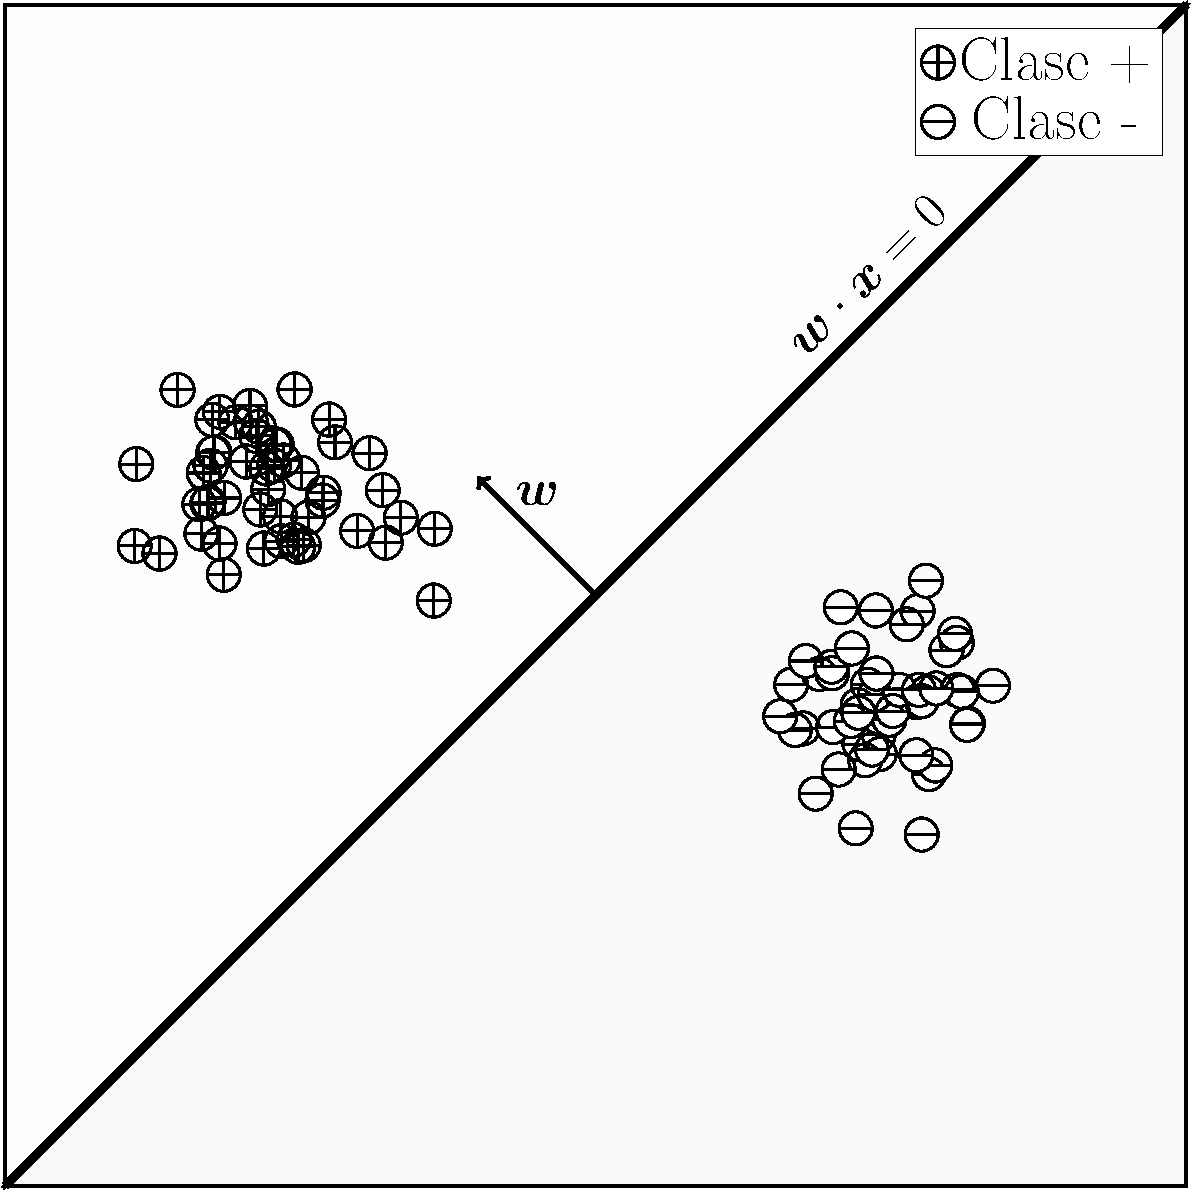
\includegraphics[width=\textwidth]{aprendizaje/hiperplano_perceptron}
%\end{column}
%\end{columns}
%
%\end{frame}
%
%\begin{frame}
%\frametitle{Perceptrón: Entrenamiento}
%\centering
%   \begin{tabular}{C{0.5\linewidth}C{0.5\linewidth}}
%      \uncover<1->{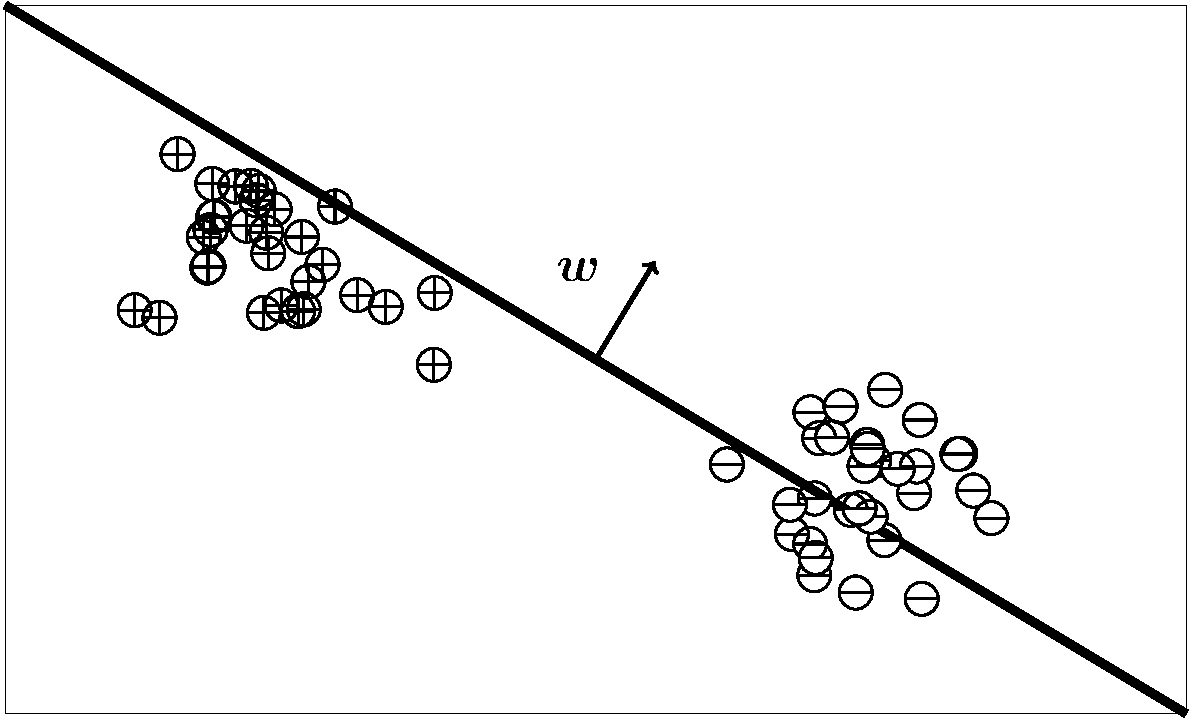
\includegraphics[width=0.35\textwidth]{aprendizaje/hiperplano_perceptron_entrenamiento1}} &    \uncover<2->{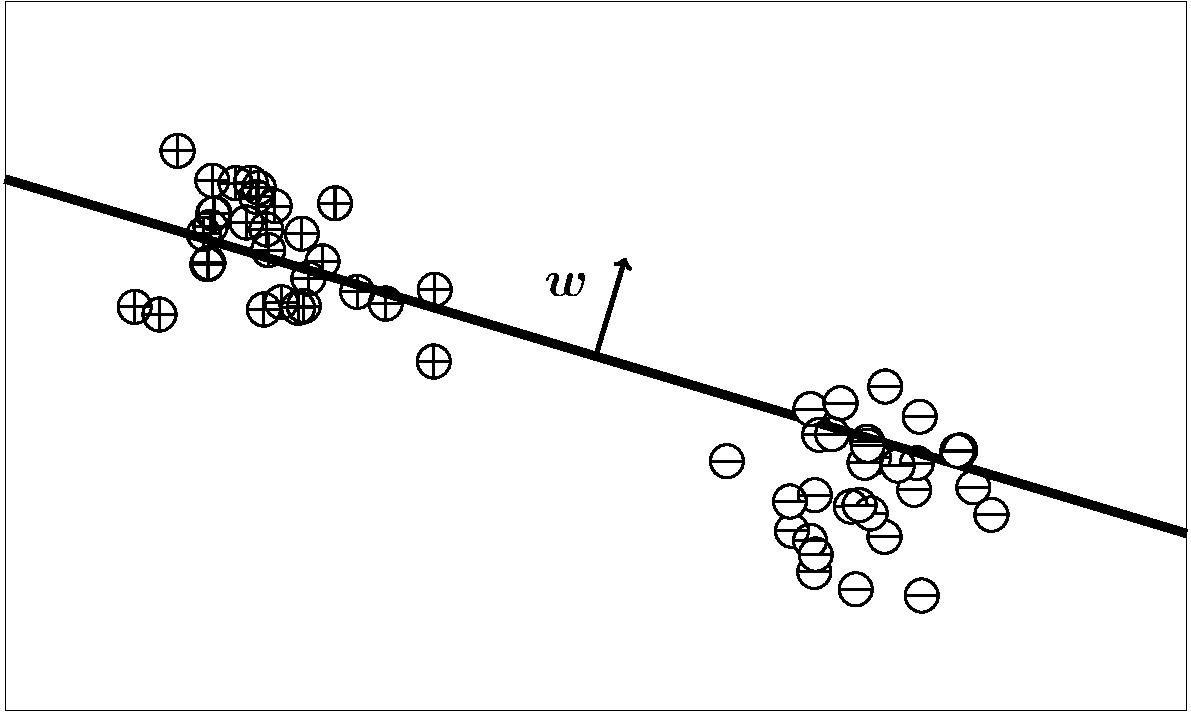
\includegraphics[width=0.35\textwidth]{aprendizaje/hiperplano_perceptron_entrenamiento2}}  \\
%      \uncover<3->{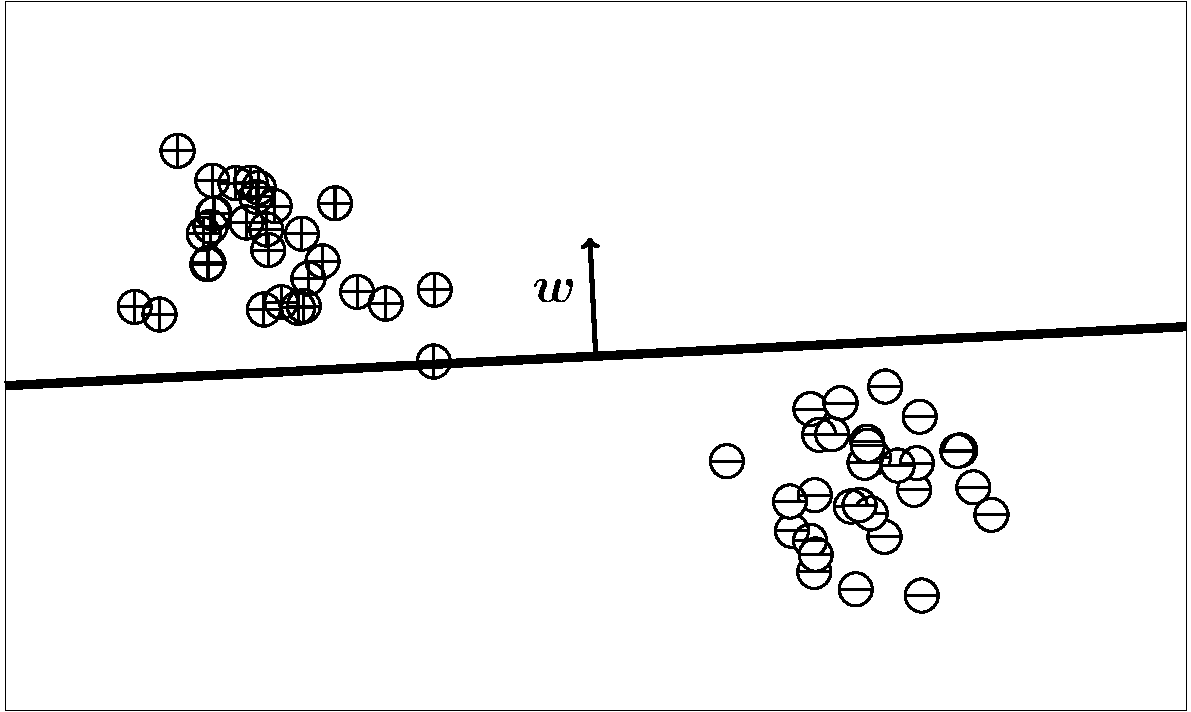
\includegraphics[width=0.35\textwidth]{aprendizaje/hiperplano_perceptron_entrenamiento3}} &    \uncover<4->{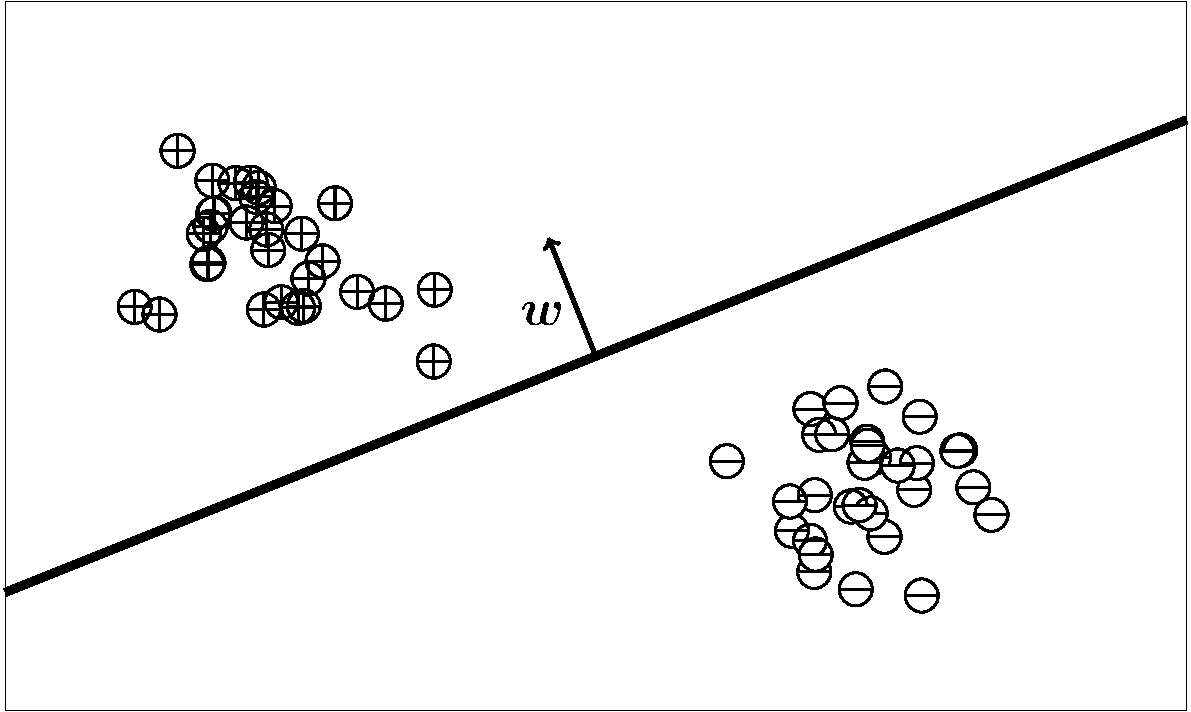
\includegraphics[width=0.35\textwidth]{aprendizaje/hiperplano_perceptron_entrenamiento4}}  
%\end{tabular}
%   
%\end{frame}


%\begin{frame}
%\frametitle{Superficies de separación: ARREGLAR IMAGENES 2 y 3 Distintas}
%\centering
%   \begin{tabular}{C{0.5\linewidth}C{0.5\linewidth}}
%      \includegraphics<1>[width=0.5\textwidth]{aprendizaje/lineal_1} 
%      \includegraphics<2->[width=0.5\textwidth]{aprendizaje/lineal_2} 
%      &    
%      \includegraphics<1>[width=0.5\textwidth]{aprendizaje/no_lineal_1} 
%      \includegraphics<2->[width=0.5\textwidth]{aprendizaje/no_lineal_2}
%      \\
%      [-1ex] Linealmente separable & No linealmente separable \\
%      \uncover<3>{ 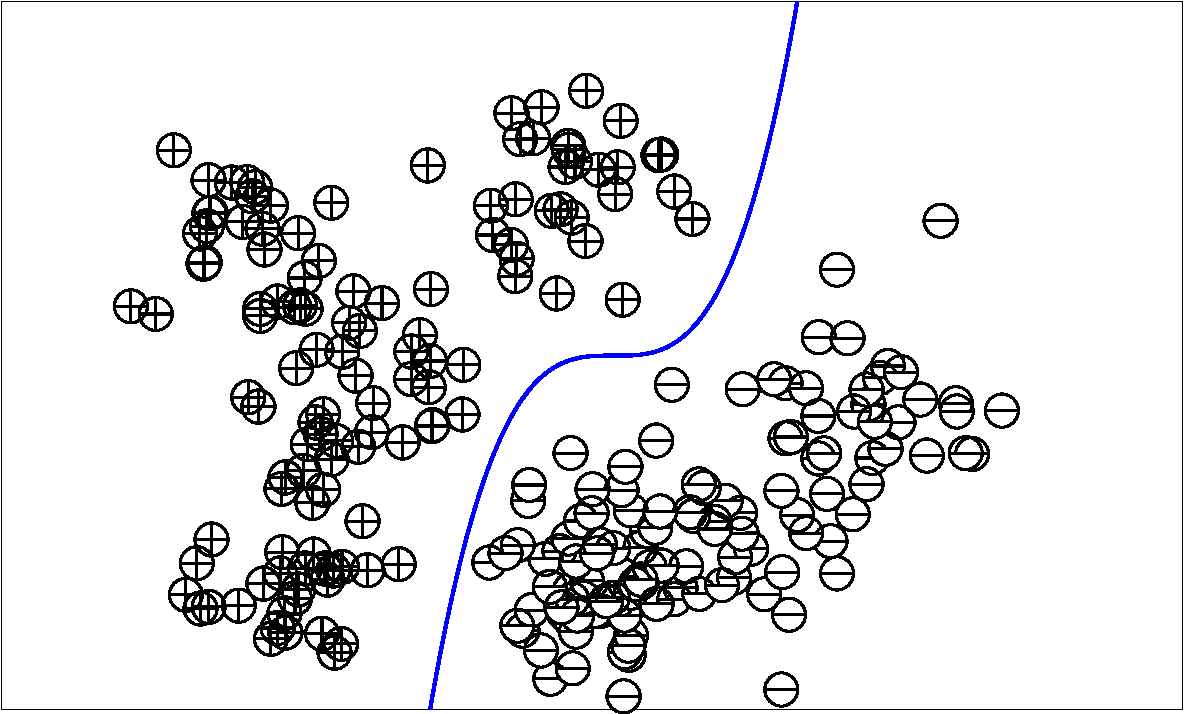
\includegraphics[width=0.5\textwidth]{aprendizaje/no_lineal_superficie_no_lineal}}
%      &    
%      \uncover<3>{ 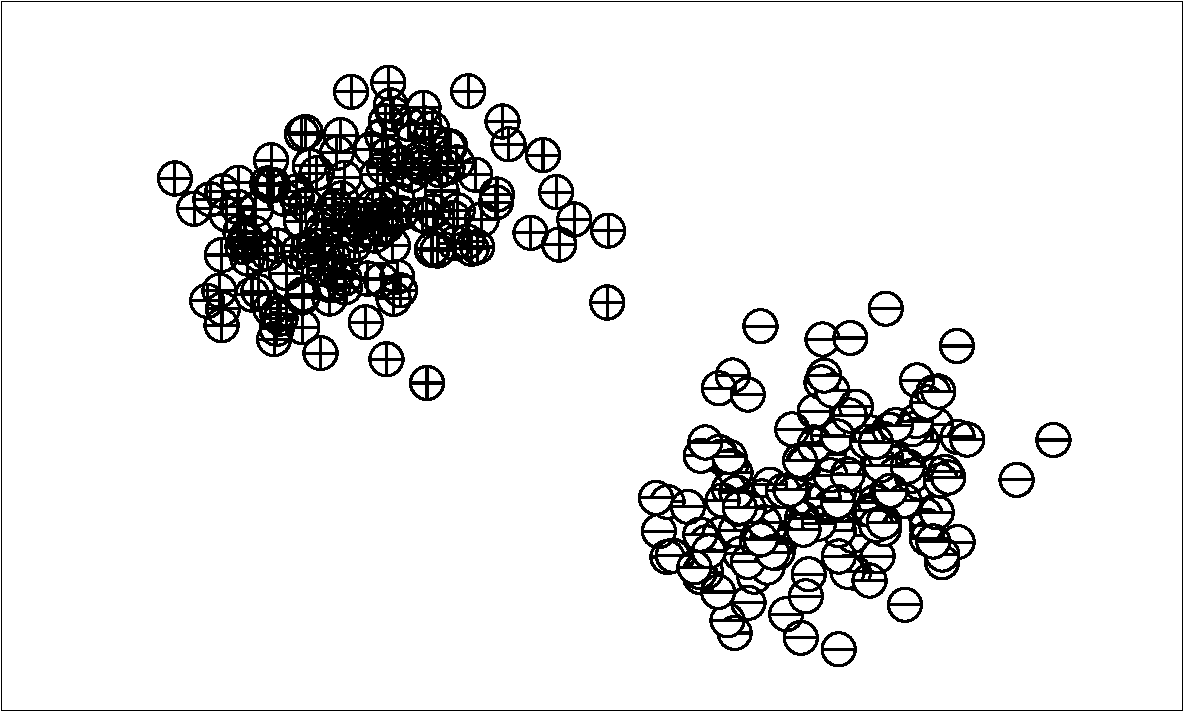
\includegraphics[width=0.5\textwidth]{aprendizaje/no_lineal_transformacion} }
%      \\
%      [-1ex]\uncover<3>{Superficie no lineal} & \uncover<3>{Otra representación}
%      \end{tabular}
%\end{frame}


%\begin{frame}
%\frametitle{Error $\rightarrow$ Experimentos de clasificación}
%\centering
%\esquemavalidacion{0.5}
%\blockitemize{}{\item Error = Porcentaje de ejemplares mal clasificados}
%\end{frame}

%\begin{frame}
%\frametitle{Entrenamiento = Minimizar Error: CAMBIAR EL PITUTO}
%\centering
%\begin{columns}
%
%\begin{column}{0.5\textwidth}
%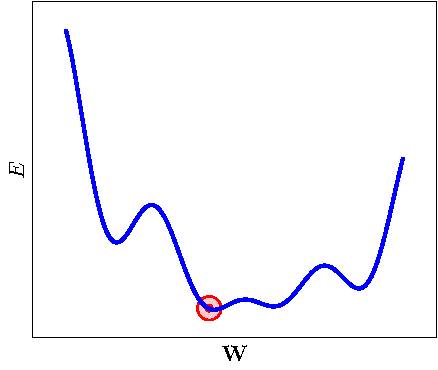
\includegraphics[width=\textwidth]{aprendizaje/error_prueba} 
%\blockitemize{}{\item Error de entrenamiento vs Parámetros}
%\end{column}
%\begin{column}{0.5\textwidth}
%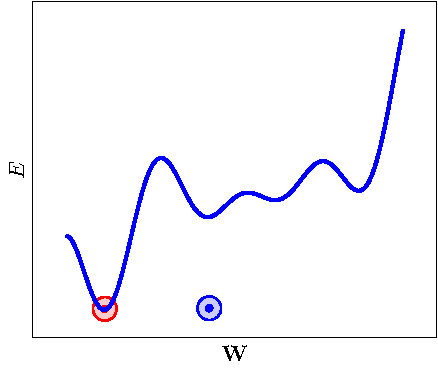
\includegraphics[width=\textwidth]{aprendizaje/error_entrenamiento} 
%\blockitemize{}{\item Error de Prueba vs Parámetros}
%\end{column}
%
%\end{columns}
%\end{frame}




% SVM

%
%\begin{frame}
%\frametitle{SVM + Márgenes Suaves}
%\centering
%   \begin{tabular}{C{0.5\linewidth}C{0.5\linewidth}}
%      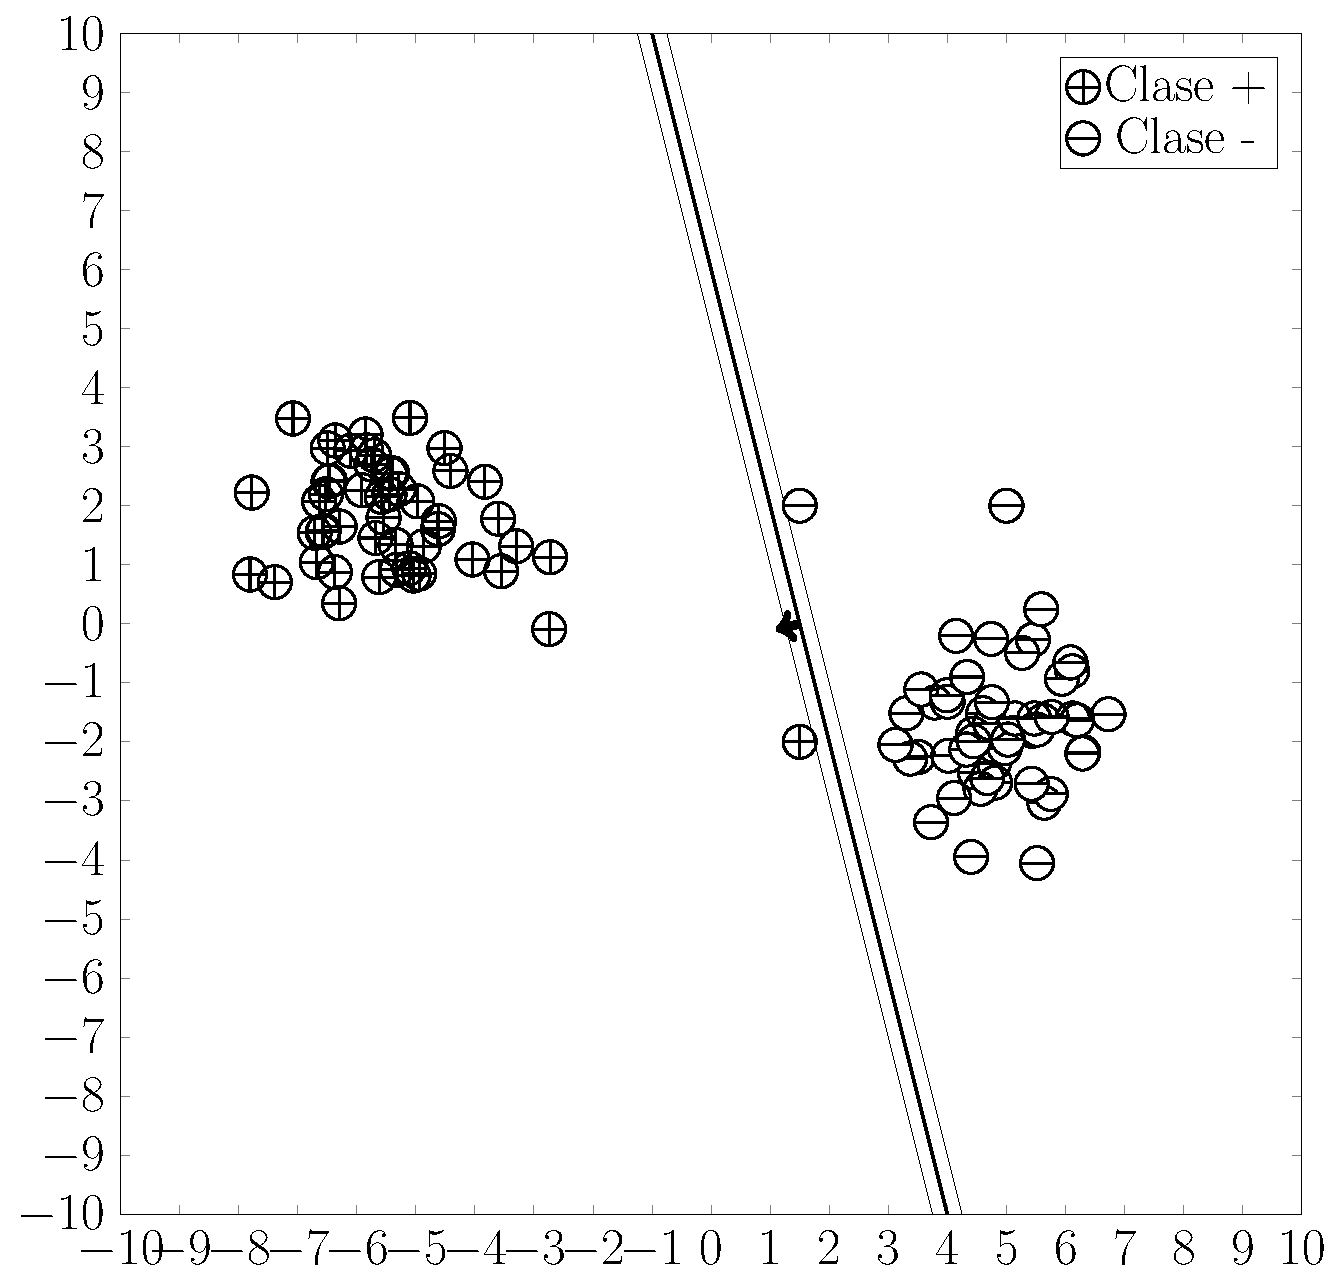
\includegraphics[width=0.5\textwidth]{aprendizaje/svm_hard} &  
%      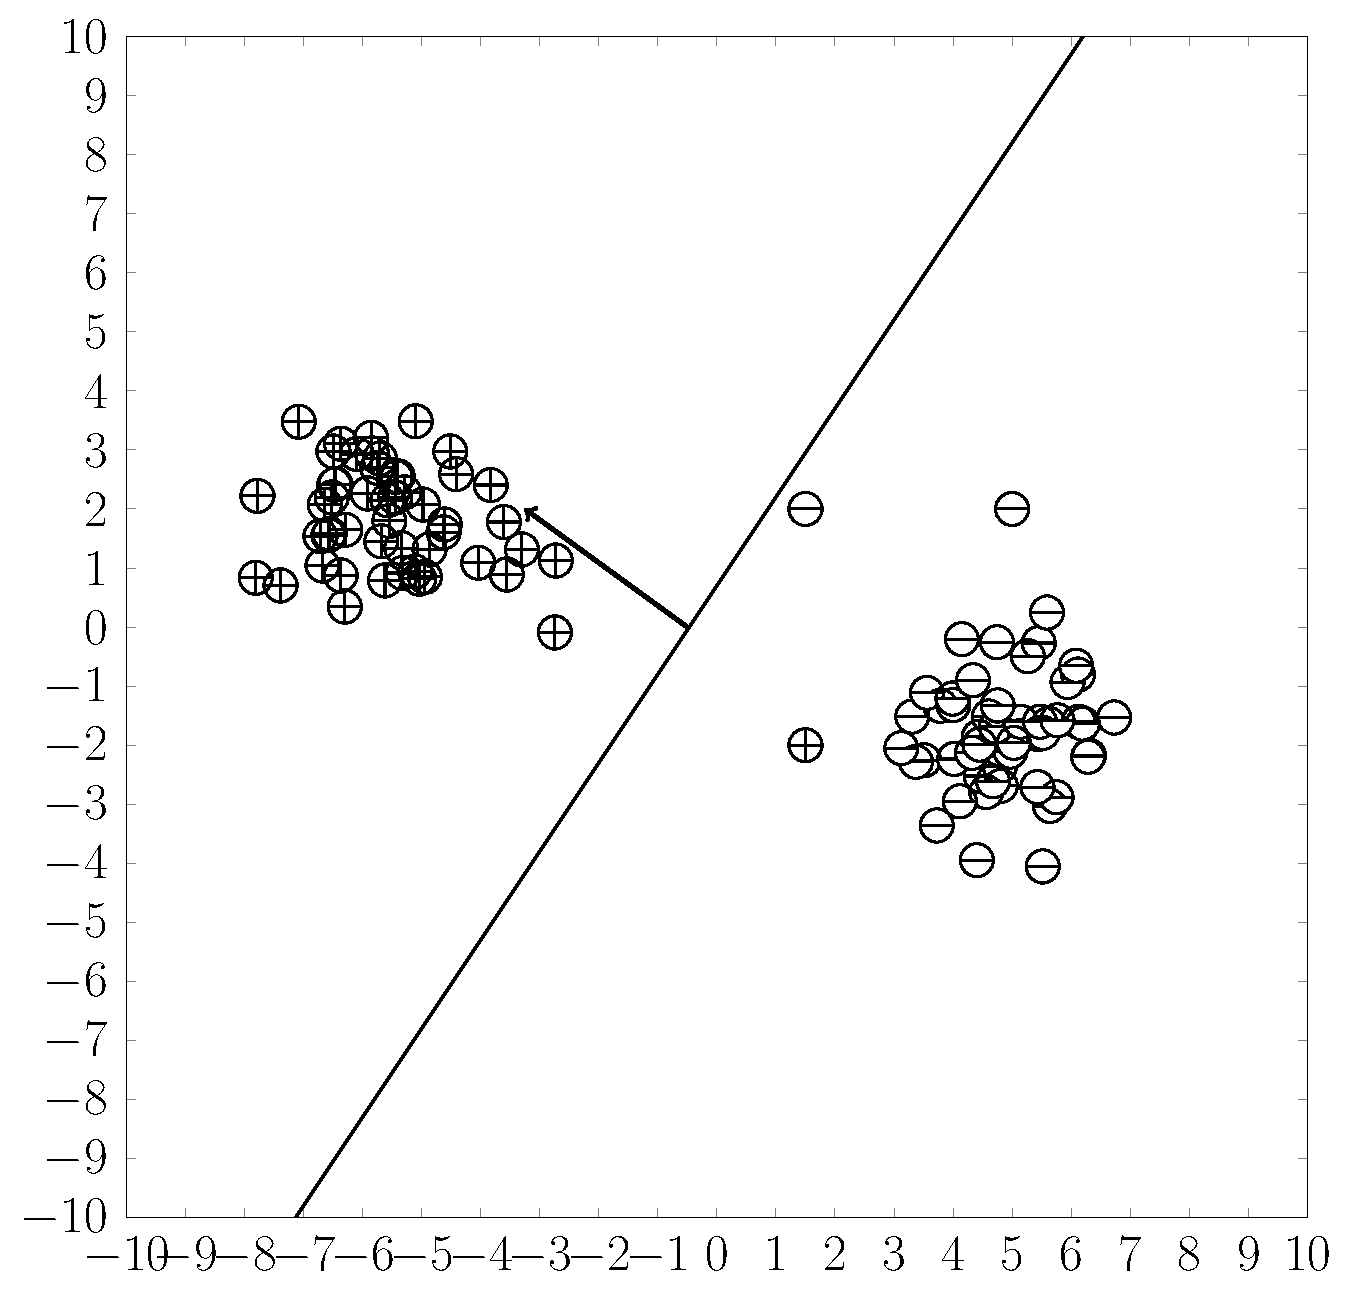
\includegraphics[width=0.5\textwidth]{aprendizaje/svm_soft}  \\
%\end{tabular}
%\vspace{-5pt}
%
%\begin{block}{}
%\vspace{-9pt}
% \begin{equation*}
% \vspace{-4pt}
%\text{Entrenamiento:} \quad \Max_{\ve{w}} \; M - c \times Error
%\end{equation*}
%\end{block}
%\end{frame}
%
%
%\begin{frame}
%\frametitle{SVM + Márgenes Suaves + Kernels}
%\centering
%   \begin{tabular}{C{0.5\linewidth}C{0.5\linewidth}}
%      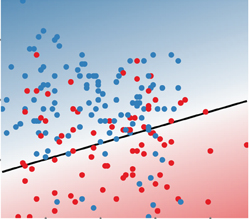
\includegraphics[width=0.5\textwidth]{aprendizaje/svm_kernel_linear} &  
%      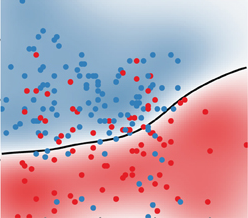
\includegraphics[width=0.5\textwidth]{aprendizaje/svm_kernel_gaussian}  \\
%      [-1ex] Kernel Lineal & Kernel Gaussiano
%\end{tabular}

%\begin{tikzpicture}
%\pgfplotsset{ticks=none}
%\begin{axis}[width=\textwidth,height=90  ,transform shape]
%\addplot[domain=-50:50, samples=200,ultra thick,color= blue]{0.02*x*x};
%\end{axis}
%\end{tikzpicture}

%\blockitemize{}{\item Función de error convexa}

%\end{frame}

%\subsection{Redes neuronales }
%\begin{frame}\frametitle{Redes neuronales artificiales}
%\centering
%
%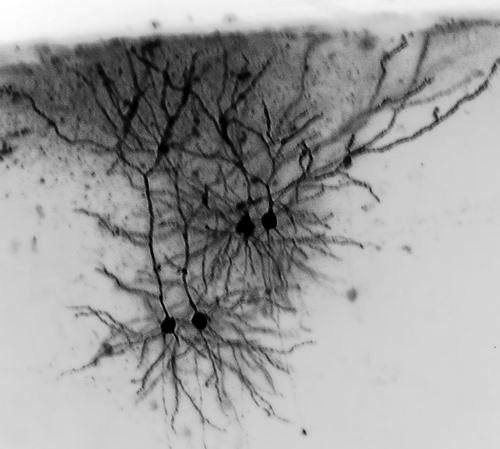
\includegraphics[width=0.7\textwidth]{aprendizaje/biological_mouse} 
%\blockitemize{}{\item Porción de red neuronal de un ratón}
%
%%
%%\begin{columns}
%%
%%\begin{column}{0.5\textwidth}
%%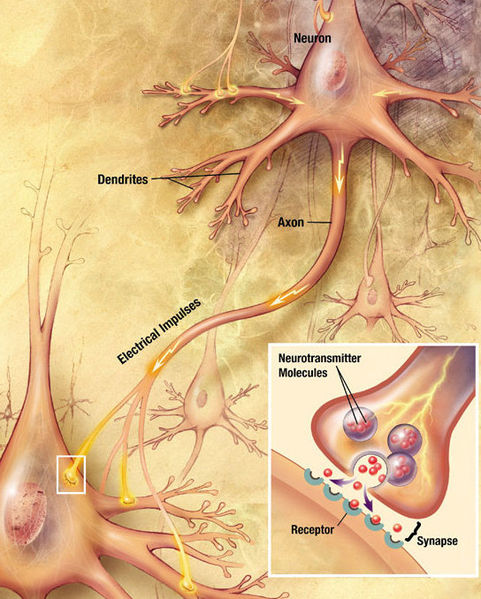
\includegraphics[width=\textwidth]{aprendizaje/histologia} 
%%\blockitemize{}{\item  Esquema red neuronal}
%%\end{column}
%%\begin{column}{0.5\textwidth}
%%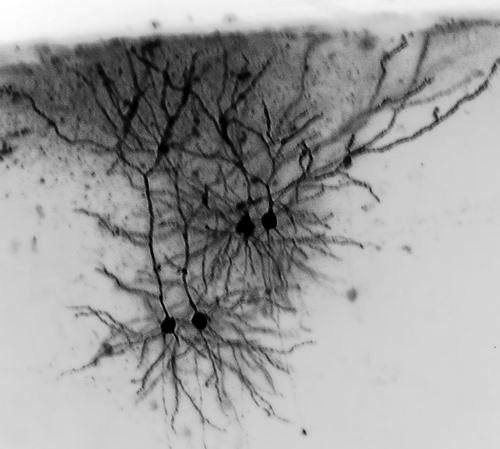
\includegraphics[width=\textwidth]{aprendizaje/biological_mouse} 
%%\blockitemize{}{\item Porción de red neuronal de un ratón}
%%\end{column}
%%
%%\end{columns}
%\end{frame}


%\begin{myframe}
%\frametitle{FF: Funciones}
%
%\centering
%\begin{columns}
%
%\begin{column}{0.53\textwidth}
%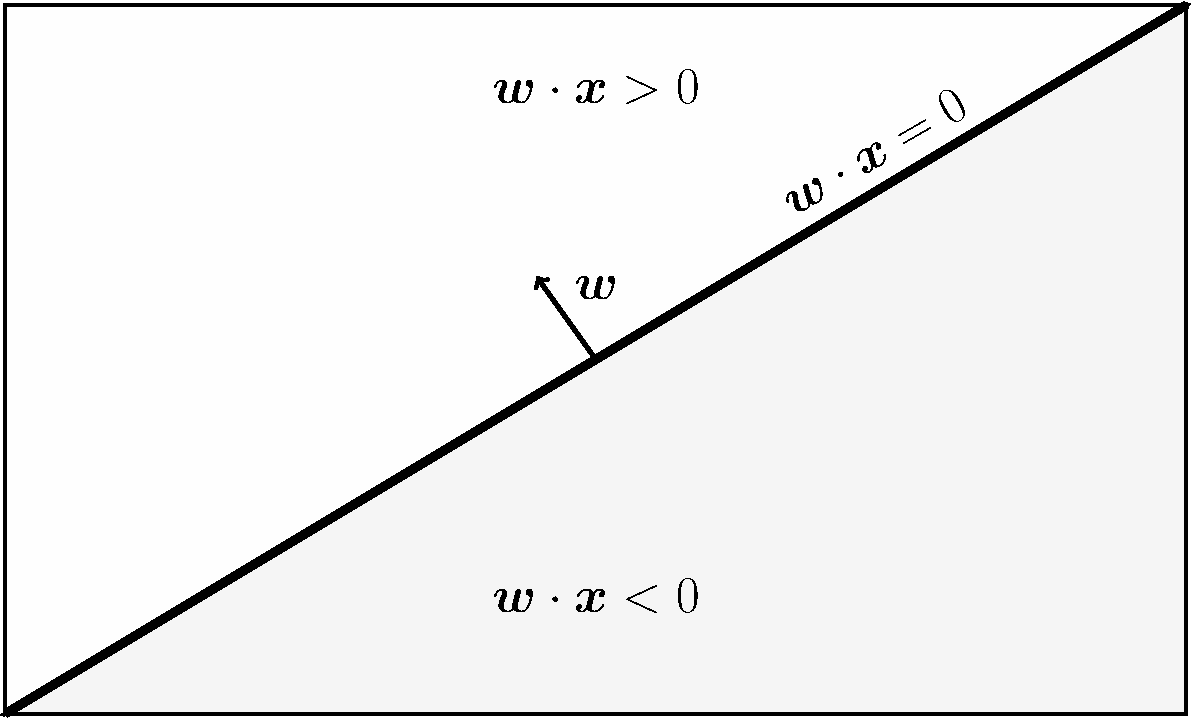
\includegraphics[width=\textwidth]{aprendizaje/hiperplano_regiones_2} 
%\blockitemize{Elección usual}{
%  \item  Hiperplano: $h(\xv)= \wv \cdot \xv$
%  \item  Sigmoide : $tanh(x)= \frac{1-e^{-2x}}{1+e^{-2x}}$
%  \item $f_i=g_i=f(\xv)= tanh(h(\xv))$ 
%  \item Parámetro: $\wv$
%}
%\end{column}
%\begin{column}{0.5\textwidth}
%\centering
%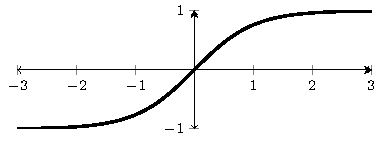
\includegraphics[width=\textwidth]{aprendizaje/tanh_angosta} \\
%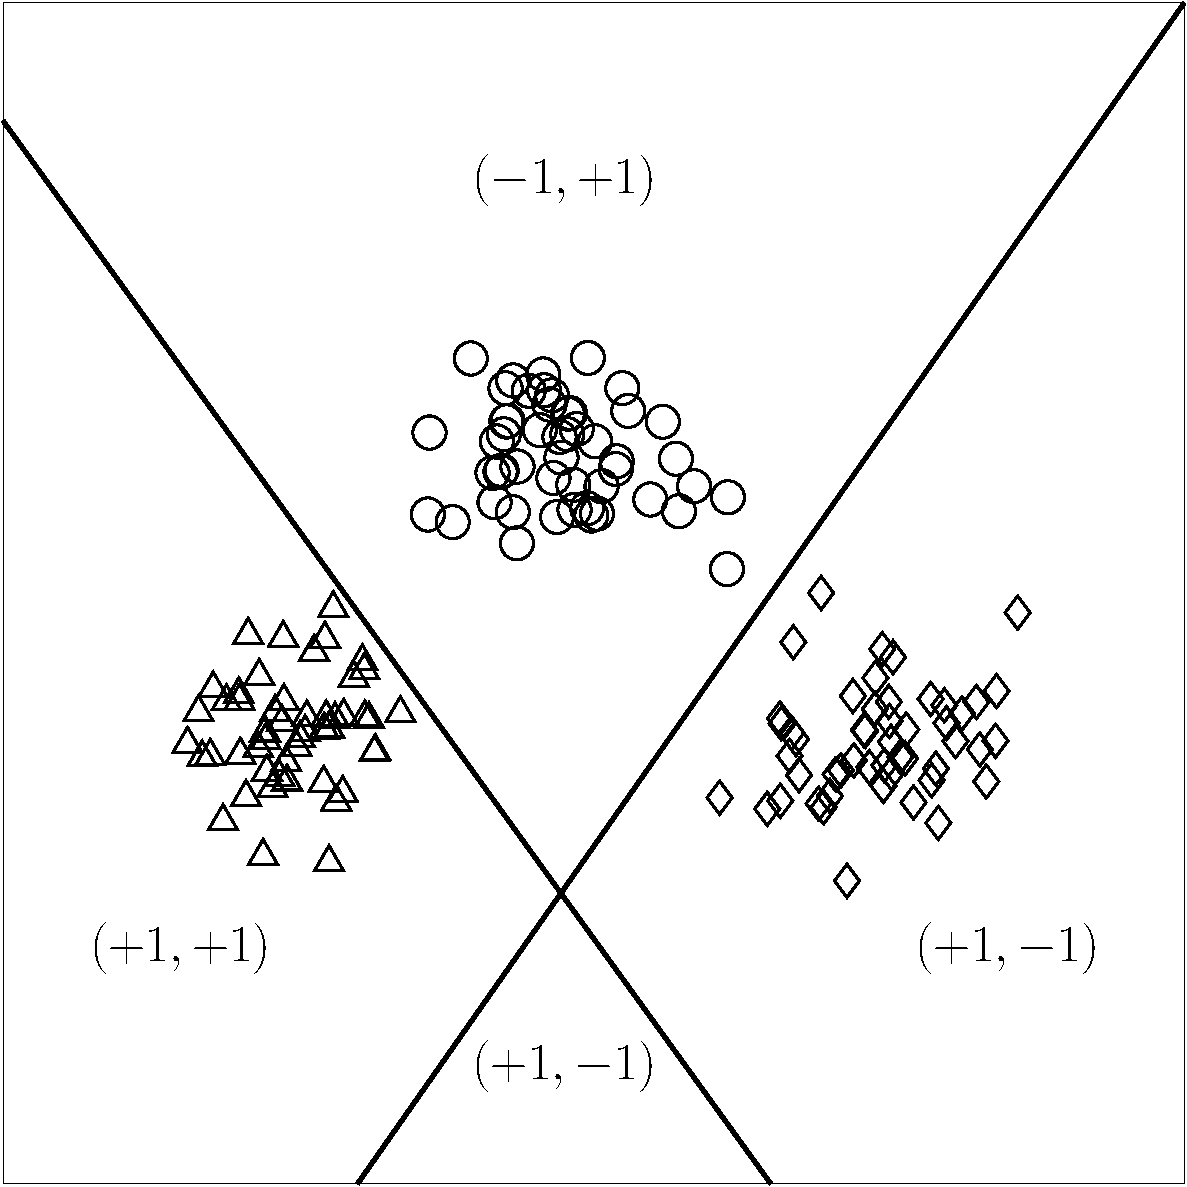
\includegraphics[width=0.9\textwidth]{aprendizaje/codificacion_ocultas_hiperplano} 
%\end{column}
%\end{columns}
%\end{myframe}


%\begin{myframe}
%\frametitle{FF: Entrenamiento}
%\centering
%
%\begin{columns}
%\begin{column}{0.7\textwidth}
%\centering
%\includegraphics<1>[width=\textwidth]{aprendizaje/entrenamiento_backpropagation} 
%\includegraphics<2>[width=\textwidth]{aprendizaje/entrenamiento_backpropagation1} 
%\includegraphics<3>[width=\textwidth]{aprendizaje/entrenamiento_backpropagation2} 
%\includegraphics<4>[width=\textwidth]{aprendizaje/entrenamiento_backpropagation3} 
%\includegraphics<5>[width=\textwidth]{aprendizaje/entrenamiento_backpropagation4} 
%\end{column}
%\begin{column}{0.4\textwidth}
%\centering
%\blockitemize{Regla actualización:}{
%\item $\derivative{E}{\ve{W}}$ = Dirección p/ suba error
%\item $-\derivative{E}{\ve{W}}$ = Dirección de p/ baje error
%\item Idea: dar pasos en dirección $-\derivative{E}{\ve{W}}$
%\item $\alpha$ = magnitud del paso
%\item $\ve{W} := \ve{W} - \alpha \derivative{E}{\ve{W}}$
%}
%\end{column}
%\end{columns}
%
%\end{myframe}





